Obiettivo del controllo orbitale drag-free è la cancellazione delle forze non
gravitazionali agenti sul satellite per rendere il moto del centro di massa del
satellite dovuto con accettabile approssimazione esclusivamente alle forze
gravitazionali. L'accelerazione del centro di massa del satellite è descritta
dalle seguenti relazioni (tutte le coordinate sono espresse nel riferimento
corpo):

\begin{equation}
\components{\dot{v}}(t) = \components{g}(\components{r}(t))+
\frac{R_b(\quat{q})(-\components{F_d}(t)+\components{F_t}(t))}{m},
\components{v(0)=v_	0}
\end{equation}
dove $\components{F_d}$ sono le forze non gravitazionali (principalmente
aerodinamiche in orbita bassa) e $\components{F_t}$ sono le forze di comando
dovute ai propulsori.

Il controllo drag-free è soddisfatto quando la seguente relazione è soddisfatta:

\begin{equation}
\components{a}(t) = \frac{(- \components{F_d}(t) + \components{F_t}(t))}{m}=0
\end{equation}
ovvero l'accelerazione residua dovuta a componenti non gravitazionali
($\components{a}$) è nulla.

L'architettura prescelta per la compensazione delle forze suddette è basata 
sull' embedded model, essa è rappresentata in figura \ref{fig:orbit_control} e
corrisponde alle seguenti equazioni (introdurremo l'equazione del comando
nella prossima sezione):

\begin{IEEEeqnarray}{rCl}
	x(i+1)&=&(1-\beta)x(i) + \beta(d(i)+w_0(i)+u(i))\nonumber\\
	y(i)&=&x(i)+e(i) = y_m(i)+ e(i)
\end{IEEEeqnarray}
Di seguito una descrizione delle componenti dell'architettura di controllo e
dei parametri delle equazioni:
\begin{description}
\item[Dinamica Controllabile:] Descrive la dinamica tra comando e misura, deve
catturare le dinamiche ad alta frequenza il più vicino possibile alla più alta
componente in frequenza dei disturbi da cancellare.
\item[Dinamica del Disturbo:] Dinamica rappresentante il disturbo e modellata su
base statistica.
\item[Beta ($\beta$):] Compreso tra zero e 1 serve a modellare il ritardo
ingresso uscita tra l'applicazione del comando e la misura
\item[Disturbi prevedibili ($x_{d1} = a_{d} +d_{a}$):] Rappresentano la somma di
accelerazioni non gravitazionali ($a_{d}$) e disturbi sull'accelerometro
($d_{a}$, bias e/o drift)
\item[Disturbo dei propulsori ($w_0$):] Rumore bianco rappresentante la
caratteristica del rumore prodotto dai propulsori
\item[Uscita del sistema ($y$):] \'{E} la misura rilevata dall'accelerometro
corrotta da eventuali disturbi e da cui sottraendo l'uscita del modello ($y_m$)
è possibile ricavare l'errore di modello utilizzato per aggiornare lo stato del
modello
\end{description} 

\begin{figure}
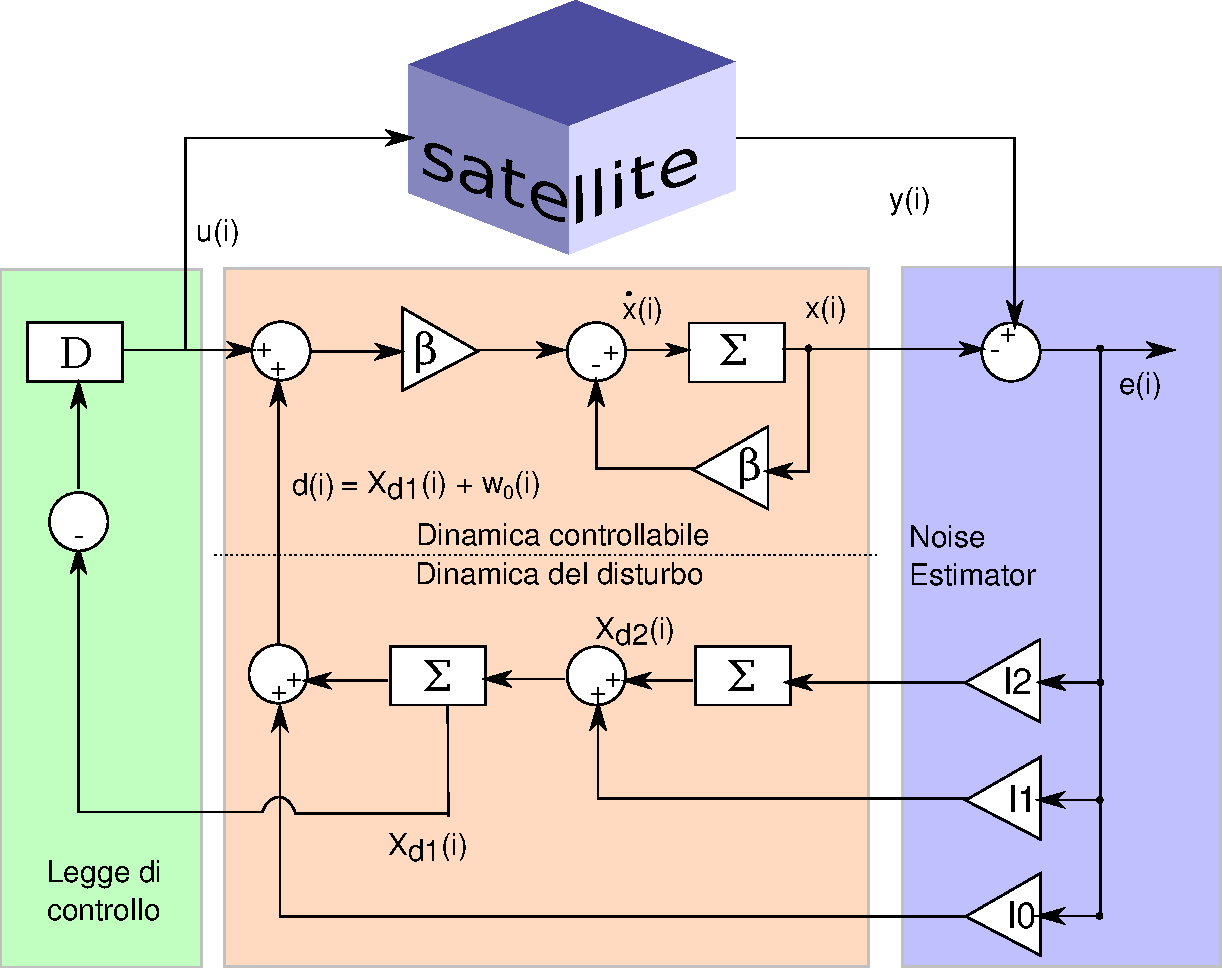
\includegraphics[width=\textwidth]{control/orbit_control/images/block-diagram.pdf}
\caption{Architettura del controllo}
\label{fig:orbit_control}
\end{figure}

